\documentclass{beamer}

\usetheme{Boadilla}

\usepackage{xifthen}
\usepackage{tikz}
\usetikzlibrary{calc}

\title{Graphes et Algorithmes}
\author{loig.jezequel@univ-nantes.fr}
\date{}

\AtBeginSection[]{
    \begin{frame}
        \vfill
        \centering
        \begin{beamercolorbox}[sep=8pt,center,shadow=true,rounded=true]{title}
            \usebeamerfont{title}\insertsectionhead\par%
        \end{beamercolorbox}
        \vfill
    \end{frame}
}

\newcommand{\enavant}[1]{\textcolor{red}{#1}}

% defs, exercices, etc
\newcommand{\notation}[2][]{
    \begin{block}{Notation\ifthenelse{\NOT\isempty{#1}}{~: #1}{}}
        #2
    \end{block}
}

\renewcommand{\definition}[2][]{
    \begin{block}{Définition\ifthenelse{\NOT\isempty{#1}}{~: #1}{}}
        #2
    \end{block}
}

\newcommand{\exercice}[2][]{
    \begin{exampleblock}{Exercice\ifthenelse{\NOT\isempty{#1}}{~: #1}{}}
        #2
    \end{exampleblock}
}

\newcommand{\proposition}[2][]{
    \begin{alertblock}{Proposition\ifthenelse{\NOT\isempty{#1}}{~: #1}{}}
        #2
    \end{alertblock}
}

\newcommand{\remarque}[2][]{
    \begin{alertblock}{Remarque\ifthenelse{\NOT\isempty{#1}}{~: #1}{}}
        #2
    \end{alertblock}
}

% notations
\newcommand{\arcs}{E}
\newcommand{\arc}{e}
\newcommand{\arcvers}[1]{t(#1)}
\newcommand{\arcdepuis}[1]{f(#1)}
\newcommand{\sommets}{V}
\newcommand{\sommet}{v}
\newcommand{\sommetb}{v'}
\newcommand{\pre}[1]{#1^-}
\newcommand{\suc}[1]{#1^+}
\newcommand{\graphe}{G}
\newcommand{\graphefunc}{\mathcal{G}}
\newcommand{\graphedef}{\graphe{} = (\sommets{}, \arcs{})}
\newcommand{\taille}[1]{|#1|}
\newcommand{\adjmat}[1]{\mathcal{A}_{#1}}
\newcommand{\adjmatelem}{a_{ij}}
\newcommand{\incmat}[1]{\mathcal{I}_{#1}}
\newcommand{\incmatelem}{\textrm{\sc i}_{ij}}
\newcommand{\voisins}[1]{N(#1)}
\newcommand{\degnot}{d}
\newcommand{\degre}[1]{\degnot{}(#1)}
\newcommand{\dege}[1]{\degnot{}^-(#1)}
\newcommand{\degs}[1]{\degnot{}^+(#1)}
\newcommand{\relation}{R}
\newcommand{\ensemble}{X}

% dessins
\newcommand{\shiftdraw}[4]{\draw[shorten >=7pt, shorten <=7pt, -latex] let \p1 = (#1), \p2 = (#2) in [shift={(#3, #4)}] (\p1) -- (\p2)}

\begin{document}

    \frame{
        \maketitle{}
    }

    \section{Présentation du cours}

\frame{
    \frametitle{Organisation du cours}

    \begin{block}{Organisation des séances}
        \begin{description}
            \item[CM~:] notions de base sur les graphes, présentation d'algorithmes classiques, exemple de présentation
            \item[TD~:] travail de recherche par groupe sur une application des graphes ou un sujet théorique plus avancé, présentation au reste de la classe
        \end{description}
    \end{block}

    \begin{block}{Évaluation}
        \begin{description}
            \item[50\%] tests sur le cours en début de séances
            \item[50\%] présentation des sujets de TD
        \end{description}
    \end{block}
}

\frame{
    \frametitle{Pourquoi étudier les graphes}

    \begin{block}{Graphe}
        Outil de \enavant{modélisation} permettant de représenter les relations entre les éléments d'un ensemble fini :
        \begin{itemize}
            \item routes et distances entre villes,
            \item liens hypertext entre pages web,
            \item etc
        \end{itemize}
    \end{block}

    \begin{block}{Algoritmes}
        Pour analyser les relations représentées par un graphe :
        \begin{itemize}
            \item trouver le plus court trajet entre deux villes,
            \item étudier les groupes sociaux sur internet,
            \item etc
        \end{itemize}
    \end{block}
}

\frame{
    \frametitle{Exemple d'application~: théorème des 4 couleurs}
    \hspace*{-0.5cm}\includegraphics[width=12cm]{1-quatrecouleurs.jpg}
}

\frame{
    \frametitle{Exemple d'application~: sortir d'un labyrinthe}
    \hspace*{-0.5cm}\includegraphics[width=12cm]{2-lab.jpg}
}

\frame{
    \frametitle{Exemple d'application~: recherche d'itinéraire}
    \hspace*{-0.5cm}\includegraphics[width=12cm]{3-map.jpg}
}

\frame{
    \frametitle{Exemple d'application~: représentation du web}
    \hspace*{-0.5cm}\includegraphics[width=12cm]{4-carteduweb.jpg}
}

\frame{
    \frametitle{Exemple d'application~: réseaux neuronaux}
    \hspace*{-0.5cm}\includegraphics[width=12cm]{5-neuralnetwork.jpg}
}

\frame{
    \frametitle{Sujets de recherche}

    \begin{enumerate}
        \item Représenter graphiquement les grands graphes
        \item Systèmes multi-agents~: exploration collaborative d'un graphe
        \item Recherche de chemins, algorithme A*
        \item Construire la carte d'internet
        \item Marches aléatoires sur les graphes
        \item Graphes planaires et mineurs exclus
        \item Graphes petit-mondes
        \item Réécriture de graphes
        \item Graphes et recommandation "top-N"
        \item Hypergraphes
    \end{enumerate}
}

    \section{Définitions de base}

\frame{
    \frametitle{Graphe}

    \definition{%
        Un graphe est est un couple $\graphedef{}$ avec~:
        \begin{itemize}
            \item $\sommets{}$ un ensemble \enavant{fini} de sommets,
            \item $\arcs{} \subseteq \sommets{}\times\sommets{}$ un ensemble \enavant{fini} d'arrêtes.
        \end{itemize}%
    }

    \uncover<2->{
        \only<1-2>{%
            \exercice{%
                Soit un graphe $\graphedef{}$.
                Quel est, en fonction de $\taille{\sommets{}}$, le nombre maximum d'arrêtes de $\graphe{}$ ?%
            }%
        }

        \only<3->{%
            \proposition{%
                Soit un graphe $\graphedef{}$, on a $\taille{\arcs{}} \leq \taille{\sommets{}}^2$.
            }%
        }
    }

    \uncover<4->{%
        \only<1-4>{%
            \exercice{%
                Soit un graphe $\graphedef{}$ sans sommets isolés.
                Quel est, en fonction de $\taille{\sommets{}}$, le nombre minimum d'arrêtes de $\graphe{}$ ?%
            }%
        }

        \only<5->{%
            \proposition{%
                Soit un graphe $\graphedef{}$ sans sommets isolés, on a $\taille{\arcs{}} \geq \lceil \taille{\sommets{}}/2 \rceil$

            }%
        }
    }
}

\frame{
    \frametitle{Vocabulaire}

    \definition[Successeurs]{%
        Dans un graphe $\graphedef{}$ les successeurs d'un sommet $\sommet{}\in\sommets{}$ sont les sommets $\sommetb{}\in\sommets{}$ tels que $(\sommet{}, \sommetb{})\in\arcs{}$.
    }

    \definition[Prédecesseurs]{%
        Dans un graphe $\graphedef{}$ les prédécesseurs d'un sommet $\sommet{}\in\sommets{}$ sont les sommets $\sommetb{}\in\sommets{}$ tels que $(\sommetb{}, \sommet{})\in\arcs{}$.
    }

    \definition[Graphe complet]{%
        Un graphe $\graphedef{}$ est dit complet si $\arcs{} = \sommets{}\times\sommets{}$.
    }

}

\frame{
    \frametitle{Dessiner les graphes}

    \begin{figure}
        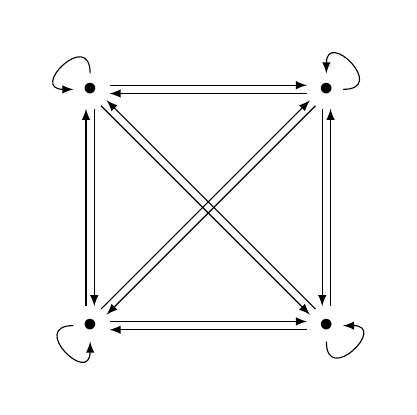
\begin{tikzpicture}
            \node (a) at (0,0) {$\bullet$};
            \node (b) at (3,0) {$\bullet$};
            \node (c) at (0,3) {$\bullet$};
            \node (d) at (3,3) {$\bullet$};

            \shiftdraw{a}{b}{0}{1.5pt};
            \shiftdraw{a}{c}{-1.5pt}{0};
            \shiftdraw{a}{d}{-1pt}{1pt};
            \draw[-latex] (a) to[in=270, out=180, looseness=5] (a);

            \shiftdraw{b}{a}{0}{-1.5pt};
            \shiftdraw{b}{c}{1pt}{1pt};
            \shiftdraw{b}{d}{1.5pt}{0};
            \draw[-latex] (b) to[in=0, out=270, looseness=5] (b);

            \shiftdraw{c}{a}{1.5pt}{0};
            \shiftdraw{c}{b}{-1pt}{-1pt};
            \shiftdraw{c}{d}{0}{1.5pt};
            \draw[-latex] (c) to[in=180, out=90, looseness=5] (c);

            \shiftdraw{d}{a}{1pt}{-1pt};
            \shiftdraw{d}{b}{-1.5pt}{0};
            \shiftdraw{d}{c}{0}{-1.5pt};
            \draw[-latex] (d) to[in=90, out=0, looseness=5] (d);
        \end{tikzpicture}
        \caption{Un graphe complet à 4 sommets}
    \end{figure}
}

\frame{
    \frametitle{Les graphes vus comme des fonctions}

    \definition[À partir des successeurs]{%
        \begin{eqnarray*}
            \graphefunc{} & : & \sommets{} \rightarrow 2^\sommets{} \\
                          &   & \sommet{} \mapsto \{ \sommetb{}~|~(\sommet{}, \sommetb{})\in \arcs{} \}
        \end{eqnarray*}
    }

    \definition[À partir des prédecesseurs]{%
        \begin{eqnarray*}
            \graphefunc{} & : & \sommets{} \rightarrow 2^\sommets{} \\
                          &   & \sommet{} \mapsto \{ \sommetb{}~|~(\sommetb{}, \sommet{})\in \arcs{} \}
        \end{eqnarray*}
    }
}

\frame{
    \frametitle{Les graphes vus comme des matrices}

    \definition[matrice d'adjacence]{%
        Soit $\graphedef{}$ un graphe.
        On pose $n=\taille{\sommets{}}$ et $\sommets{}=\{\sommet{}_1, \dots, \sommet{}_n\}$.
        La matrice d'adjacence de $\graphe{}$ est $\adjmat{\graphe{}}=(\adjmatelem{})_{1\leq i, j \leq n}$ telle que~:
        \begin{eqnarray*}
            \adjmatelem{} = 1 & \textrm{si} & (\sommet{}_i, \sommet{}_j)\in\arcs{} \\
            \adjmatelem{} = 0 & \textrm{sinon} &
        \end{eqnarray*}
    }

    \pause

    \exercice{%
        Donner la matrice d'adjacence du graphe suivant~:

        \begin{center}
        \scalebox{0.6}{%
            \begin{tikzpicture}
                \node (a) at (0,0) {$\sommet{}_3$};
                \node (b) at (3,0) {$\sommet{}_4$};
                \node (c) at (0,3) {$\sommet{}_1$};
                \node (d) at (3,3) {$\sommet{}_2$};
    
                \draw[-latex] (a) to[in=270, out=180, looseness=5] (a);
    
                \shiftdraw{b}{a}{0}{-1.5pt};
    
                \shiftdraw{c}{a}{1.5pt}{0};
                \shiftdraw{c}{d}{0}{1.5pt};
    
                \shiftdraw{d}{b}{-1.5pt}{0};
                \shiftdraw{d}{c}{0}{-1.5pt};
                \draw[-latex] (d) to[in=90, out=0, looseness=5] (d);
            \end{tikzpicture}
        }
        \end{center}
    }
}

\frame{
    \frametitle{Les graphes vus comme des matrices, suite}

    \notation{%
        Soit $\graphedef{}$ un graphe et soit $\arc{} = (\sommet{}, \sommetb{})\in\arcs{}$ une arrête, on note $\sommet{} = \arcdepuis{\arc{}}$ et $\sommetb{} = \arcvers{\arc{}}$.
    }

    \definition[matrice d'incidence]{%
        Soit $\graphedef{}$ un graphe.
        On pose $n=\taille{\sommets{}}$ et $\sommets{}=\{\sommet{}_1, \dots, \sommet{}_n\}$.
        De même, on pose $m=\taille{\arcs{}}$ et $\arcs{}=\{\arc{}_1, \dots, \arc{}_m\}$.
        La matrice d'incidence de $\graphe{}$ est la matrice $\incmat{\graphe{}} = (\incmatelem{})_{1\leq i\leq n, 1\leq j\leq m}$ telle que~:
        \begin{eqnarray*}
            \incmatelem{} = 1 & \textrm{si} & \arcdepuis{\arc{}_j} = \sommet{}_i \\
            \incmatelem{} = -1 & \textrm{si} & \arcvers{\arc{}_j} = \sommet{}_i \\
            \incmatelem{} = 0 & sinon &
        \end{eqnarray*}
    }
}

\frame{
    \frametitle{Les graphes vus comme des matrices, suite, suite}

    \exercice{%
        Donner la matrice d'incidence du graphe suivant~:
        \begin{center}
            \scalebox{0.8}{%
                \begin{tikzpicture}
                    \node (a) at (0,0) {$\sommet{}_3$};
                    \node (b) at (3,0) {$\sommet{}_4$};
                    \node (c) at (0,3) {$\sommet{}_1$};
                    \node (d) at (3,3) {$\sommet{}_2$};
        
                    \node (tmp) at (1.5,3.3) {$\arc{}_1$};
                    \node (tmp) at (1.5,2.7) {$\arc{}_2$};
                    \node (tmp) at (-0.3,1.5) {$\arc{}_3$};
                    \node (tmp) at (3.3,1.5) {$\arc{}_4$};
                    \node (tmp) at (1.5,-0.3) {$\arc{}_5$};

                    \shiftdraw{b}{a}{0}{-1.5pt};
        
                    \shiftdraw{c}{a}{1.5pt}{0};
                    \shiftdraw{c}{d}{0}{1.5pt};
        
                    \shiftdraw{d}{b}{-1.5pt}{0};
                    \shiftdraw{d}{c}{0}{-1.5pt};
                \end{tikzpicture}
            }
        \end{center}
    }

    \pause

    \remarque{%
        La représentation en matrice d'incidence ne permet pas d'avoir des arcs $\arc{}$ tels que $\arcdepuis{\arc{}} = \arcvers{\arc{}}$.
    }
}

\frame{
    \frametitle{Structures de données classiques}

    Les structures de données qu'on utilise le plus souvent pour représenter les graphes sont les suivantes~:
    \begin{itemize}
        \item matrice d'adjacence
        \item listes de successeurs
        \item listes de prédécesseurs
    \end{itemize}

    \pause

    \exercice{%
        Donner la représentation en listes de successeurs et en listes de prédecesseurs du graphe dont on a précédement donné la matrice d'adjacence.
    }

    \exercice{%
        Proposer un algorithme qui permet d'obtenir une représentation en listes de successeurs à partir d'une représentation en matrice d'adjacence.
    }
}

\frame{
    \frametitle{Voisins}

    \definition[prédecesseurs]{%
        Dans un graphe $\graphedef{}$ l'ensemble des prédécesseurs d'un sommet $\sommet{}\in\sommets{}$ est noté~:
        $$\pre{\sommet{}} = \{\sommetb{}~|~(\sommetb{},\sommet{})\in\arcs{}\}$$
    }

    \definition[successeurs]{%
        Dans un graphe $\graphedef{}$ l'ensemble des successeurs d'un sommet $\sommet{}\in\sommets{}$ est noté~:
        $$\suc{\sommet{}} = \{\sommetb{}~|~(\sommet{},\sommetb{})\in\arcs{}\}$$
    }

    \definition[voisins d'un sommet]{%
        Soit un graphe $\graphedef{}$, soit un sommet $\sommet{}\in\sommets{}$, on appelle voisins de $\sommet{}$ les sommets qui sont soit des prédécesseurs soit des successeurs de $\sommet{}$, c'est-à-dire les sommets de l'ensemble $\voisins{\sommet{}} = \pre{\sommet{}}\cup\suc{\sommet{}}$.
    }
}

\frame{
    \frametitle{Degré}

    \definition[degré entrant]{%
        Soit un graphe $\graphedef{}$, soit un sommet $\sommet{}\in\sommets{}$, le degré entrant de $\sommet{}$ est $\dege{\sommet{}} = \taille{\pre{\sommet{}}}$.
    }

    \definition[degré sortant]{%
        Soit un graphe $\graphedef{}$, soit un sommet $\sommet{}\in\sommets{}$, le degré sortant de $\sommet{}$ est $\degs{\sommet{}} = \taille{\suc{\sommet{}}}$.
    }

    \definition[degré d'un sommet]{%
        Soit un graphe $\graphedef{}$, soit un sommet $\sommet{}\in\sommets{}$, le degré de $\sommet{}$ est $\degre{\sommet{}} = \dege{\sommet{}} + \degs{\sommet{}}$.
    }

    \definition[degré d'un graphe]{%
        Soit un graphe $\graphedef{}$, le degré de $\graphe{}$ est $\degre{\graphe{}} = \max_{\sommet{}\in\sommets{}} \degre{\sommet{}}$
    }
}

\frame{
    \frametitle{Graphes et relations binaires}

    On peut représenter une relation binaire $\relation{}$ sur un ensemble fini $\ensemble{}$ par un graphe $\graphedef{}$ dont
    \begin{itemize}
        \item les sommets sont les éléments de l'ensemble~: $\sommets{} = \ensemble{}$,
        \item les arrêtes représentent la relation~: $(x, y) \in \arcs{} \Leftrightarrow x\relation{}y$.
    \end{itemize}

    Un certain nombre de caractéristiques de la relation peuvent alors se repérer visuellement sur le graphe.

    \begin{columns}
        \begin{column}{5.5cm}
            \begin{block}{Réflexivité~: $\forall x, x\relation{}x$}
                \begin{center}
                    \begin{tikzpicture}
                        \node (a) at (0,0) {$x$};
                        \draw[-latex] (a) to[in=90, out=0, looseness=5] (a);
                    \end{tikzpicture}
                \end{center}
            \end{block}
            \begin{block}{Symétrie~: $\forall x, y, x\relation{}y \Rightarrow y\relation{}x$}
                \begin{center}
                    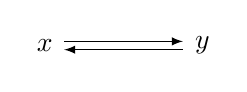
\begin{tikzpicture}
                        \node (a) at (0,0) {$x$};
                        \node (b) at (2,0) {$y$};
                        \shiftdraw{a}{b}{0}{1.5pt};
                        \shiftdraw{b}{a}{0}{-1.5pt};
                    \end{tikzpicture}
                \end{center}
            \end{block}
        \end{column}
        \begin{column}{5.5cm}
            \begin{block}{Transitivité~: $\forall x, y, z, x\relation{}y \textrm{ et } y\relation{}z \Rightarrow x\relation{}z$}
                \begin{center}
                    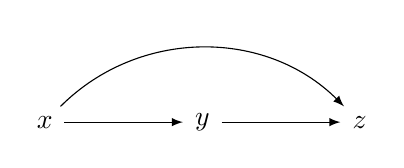
\begin{tikzpicture}
                        \node (a) at (0,0) {$x$};
                        \node (b) at (2,0) {$y$};
                        \node (c) at (4,0) {$z$};
                        \shiftdraw{a}{b}{0}{0};
                        \shiftdraw{b}{c}{0}{0};
                        \draw[-latex] (a) to[out=45, in=135] (c);
                    \end{tikzpicture}
                \end{center}
            \end{block}
        \end{column}
    \end{columns}
}

\frame{
    \frametitle{Graphes et relations binaires, suite}

    \exercice[relation d'équivalence]{%
        Comment peut-on caractériser le graphe représentant une relation d'équivalence (réflexive, symétrique et transitive) ?
    }

    \exercice[antisymmétrie]{%
        Une relation $\relation{}$ est dite antisymétrique si $\forall x, y, x\relation{}y \textrm{ et } y\relation{}x \Rightarrow x = y$.
        Comment cela se traduit-il visuellement dans un graphe ?
    }

    \exercice[relation d'ordre]{%
        Coment peut-on caractériser le graphe représentant une relation d'ordre (réflexive, antisymétrique et transitive)
    }
}

\end{document}